% id: 103-18
% book: 베이직쎈 미적분1 · 06 도함수의 활용 (3)
% section: 유형 068 시각에 대한 변화율
% figure: tikz:fig-103-18
% answer: 
% answer_source: 
% variant_level: 0 (원본 전사)
% 이 파일은 build.mjs 가 items.json 에서 만든다. 고칠 때는 items.json 을 고친다.
\smash{\raisebox{1.5mm}{\dmkichul{베이직쎈 미적분1 103쪽 18번}}}
\noindent\begin{minipage}[t]{0.58\linewidth}\vspace{0pt}\raggedright 키가 $1.6\mkern3mu \mathrm{m}$인 승규가 지면으로부터의 높이가 $4.8\mkern3mu \mathrm{m}$인 가로등 바로 밑에서 출발하여 일직선으로 초속 $2\mkern3mu \mathrm{m}$로 걷고 있다. 출발한 지 $t$초 후의 가로등 바로 밑에서부터 승규의 그림자의 앞 끝까지의 거리를 $x\mkern3mu \mathrm{m}$라 할 때, 다음에 답하시오.\end{minipage}\hfill\begin{minipage}[t]{0.4\linewidth}\vspace{0pt}\centering \resizebox{\ifdim\width>\linewidth\linewidth\else\width\fi}{!}{% 103-18(103쪽) — 높이 4.8 m 인 가로등, 키 1.6 m 인 승규, 가로등 바로 밑에서 그림자의 앞 끝까지의 거리 x m 를 나타낸 직각삼각형. 스캔 화질이 낮아 TikZ 로 다시 그림.
% 원문에 있는 것만 옮긴다: 지면 · 가로등 기둥과 등 · 빗변 · 사람 · 직각 표시 · 치수 점선(4.8 m, x m)과 화살표(1.6 m). 사람의 위치는 원문 그림의 비율 그대로이고 답이 되는 값은 적지 않는다.
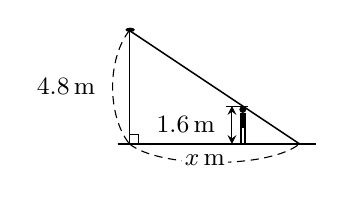
\begin{tikzpicture}[x=0.30cm, y=0.30cm, line width=0.55pt]
  % 지면과 가로등
  \draw (-0.5,0) -- (7.9,0);
  \draw (0,0) -- (0,4.8);
  \fill (0.03,4.83) ellipse (0.20 and 0.09);
  % 빛(빗변)
  \draw (0,4.8) -- (7.2,0);
  % 직각 표시
  \draw[line width=0.4pt] (0,0.40) -- (0.40,0.40) -- (0.40,0);
  % 승규
  \fill (4.80,1.455) circle (0.145);
  \fill (4.66,0.66) rectangle (4.94,1.30);
  \fill (4.68,0) rectangle (4.78,0.70);
  \fill (4.84,0) rectangle (4.94,0.70);
  % 1.6 m
  \draw[line width=0.4pt] (4.10,1.60) -- (5.00,1.60);
  \draw[densely dotted, line width=0.4pt] (4.10,0) -- (4.58,0);
  \draw[<->, >=stealth, line width=0.4pt] (4.34,0) -- (4.34,1.60);
  \node[left=1.5pt, font=\small] at (4.22,0.82) {$1.6\,\mathrm{m}$};
  % 4.8 m
  \draw[densely dashed, line width=0.4pt] (0,4.8) .. controls (-0.95,3.6) and (-0.95,1.2) .. (0,0);
  \node[left=1.5pt, font=\small] at (-0.85,2.45) {$4.8\,\mathrm{m}$};
  % x m
  \draw[densely dashed, line width=0.4pt] (0,0) .. controls (1.3,-1.05) and (5.9,-1.05) .. (7.2,0);
  \node[font=\small, fill=white, inner sep=1.2pt] at (3.20,-0.70) {$x\,\mathrm{m}$};
\end{tikzpicture}
}\end{minipage}\par
\dmsubprob{1} 출발한 지 $t$초 후의 가로등 바로 밑에서부터 승규까지의 거리를 $t$에 대한 식으로 나타내시오.
\dmsubprob{2} $x$를 $t$에 대한 식으로 나타내시오.
\dmsubprob{3} 그림자의 앞 끝이 움직이는 속도를 구하시오.
\dmsubprob{4} 그림자의 길이의 변화율을 구하시오.
